\section{Design Goal}\label{sec:goals}

The goal of the IDDR is to provide full isolation between device driver and monolithic kernel, and at the same time avoiding modifications to the device drivers. The goal of this thesis is to minimize the performance penalty because of the communication between the domains. In the IDDR implementation, we explore opportunities to minimize the overhead because of the communication module and achieve the original goals of the system such as application compatibility, transparency and strong isolation. 
\\
\subsection{Performance improvement}

IDDR is the re-implementation of the Xen driver domain, Xen driver domain is a Xen hypervisor based solution to isolate the device driver from monolithic kernel. Even though IDDR provides better robustness for operating systems, it deteriorates the performance. The reasons for the performance deterioration can be due to the introduction of an extra layer of hypervisor, data copy overhead or overhead of communication between the domains. For data intensive operations such as read and write, IDDR transfers data between hardware and the driver domain. Also, the same data is transferred between driver domain and the application domain. The extra copy from the driver domain to the application domain explains the reasons for the performance degradation. The IDDR runs the device driver in a separate domain. The application domain and driver domain communicate with each other in order to send requests and get responses from the device driver. The communication between domains adds an overhead to the system performance. Our goal is to minimize the overhead during communication between the driver domain and the application domain.

\section{Isolated Device Driver properties}
\label{sec:properties}
\subsection{Strong isolation}
One of the main goals of the IDDR is to provide strong isolation. The IDDR implementation adds an extra layer of isolation in the design which provides fault isolation between kernel and the device driver. It also adds the ability to manage individual components independently, thus, increasing the availability of the system. While exploring the opportunities to improve the performance of the IDDR, it is essential that the main goal of the IDDR is not compromised.

\subsection{Compatibility and transparency} 
The extension of existing OS structure usually results in a large number of broken applications. In the past, Microkernels required effort to retain compatibility with the existing applications~\cite{Heiser06arevirtualmachine}. In order to provide compatibility with applications, either an emulation layer was implemented~\cite{Heiser06arevirtualmachine}, or a multiserver operating system~\cite{Gefflaut00thesawmill, Tanenbaum06canwe} was built on top of a microkernel. Since the IDDR maintains compatibility between existing device drivers and applications, it is one of the basic goals of our solution to achieve the compatibility and transparency. Our solution makes sure that the performance improvement implementation will not require any changes in the device driver and the application to run the system.

\pagebreak

\section{System overview}\label{overview}
The architectural overview of the system is presented in Figure~\ref{fig:overview} .
\begin{figure}[!ht]
\centering
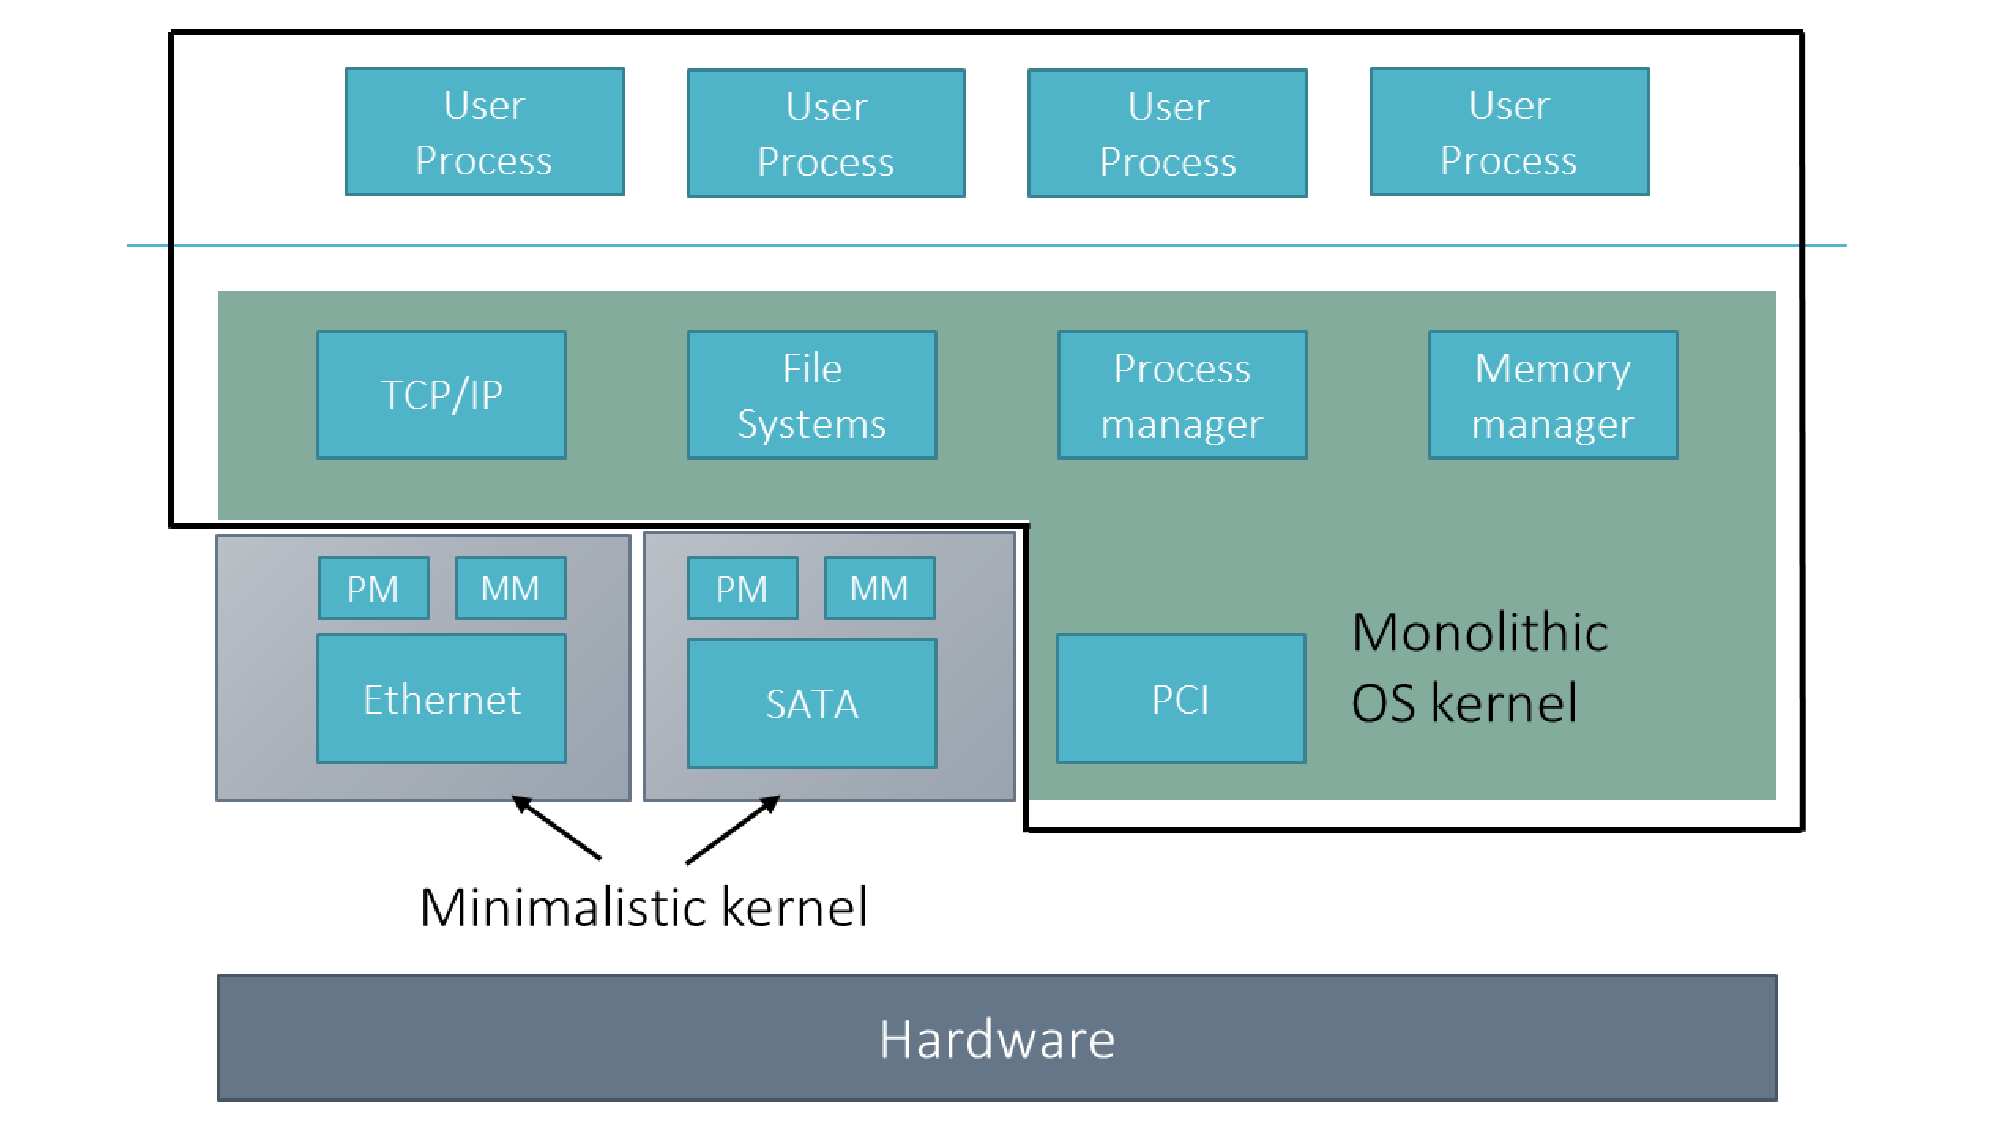
\includegraphics[scale=.5]{IDDRoverview}
\caption{Overview}
\label{fig:overview}
\end{figure}
An overview of the architecture shows that the IDDR partitions an existing kernel into multiple independent components. The user applications and Linux kernel run in a domain called as the \textit{application domain}. The device driver which needs to be isolated from the kernel, executes in the separate domain called as the \textit{driver domain}. Since in the IDDR implementation, a device driver cannot run standalone in a separate domU, hence the \textit{driver domain} runs a minimalistic kernel with the device driver. The \textit{driver domain} does not run any applications. The application domain is dedicated to the core system tasks such as process management, scheduling, user memory management, and IPC. The sole task of driver domain is to handle requests coming from the user processes managed by the application domain.
\pagebreak

\section{System components}\label{components}
3 main components of the design are Front end driver, Back end driver, Communication module.
\begin{figure}[!ht]
\centering
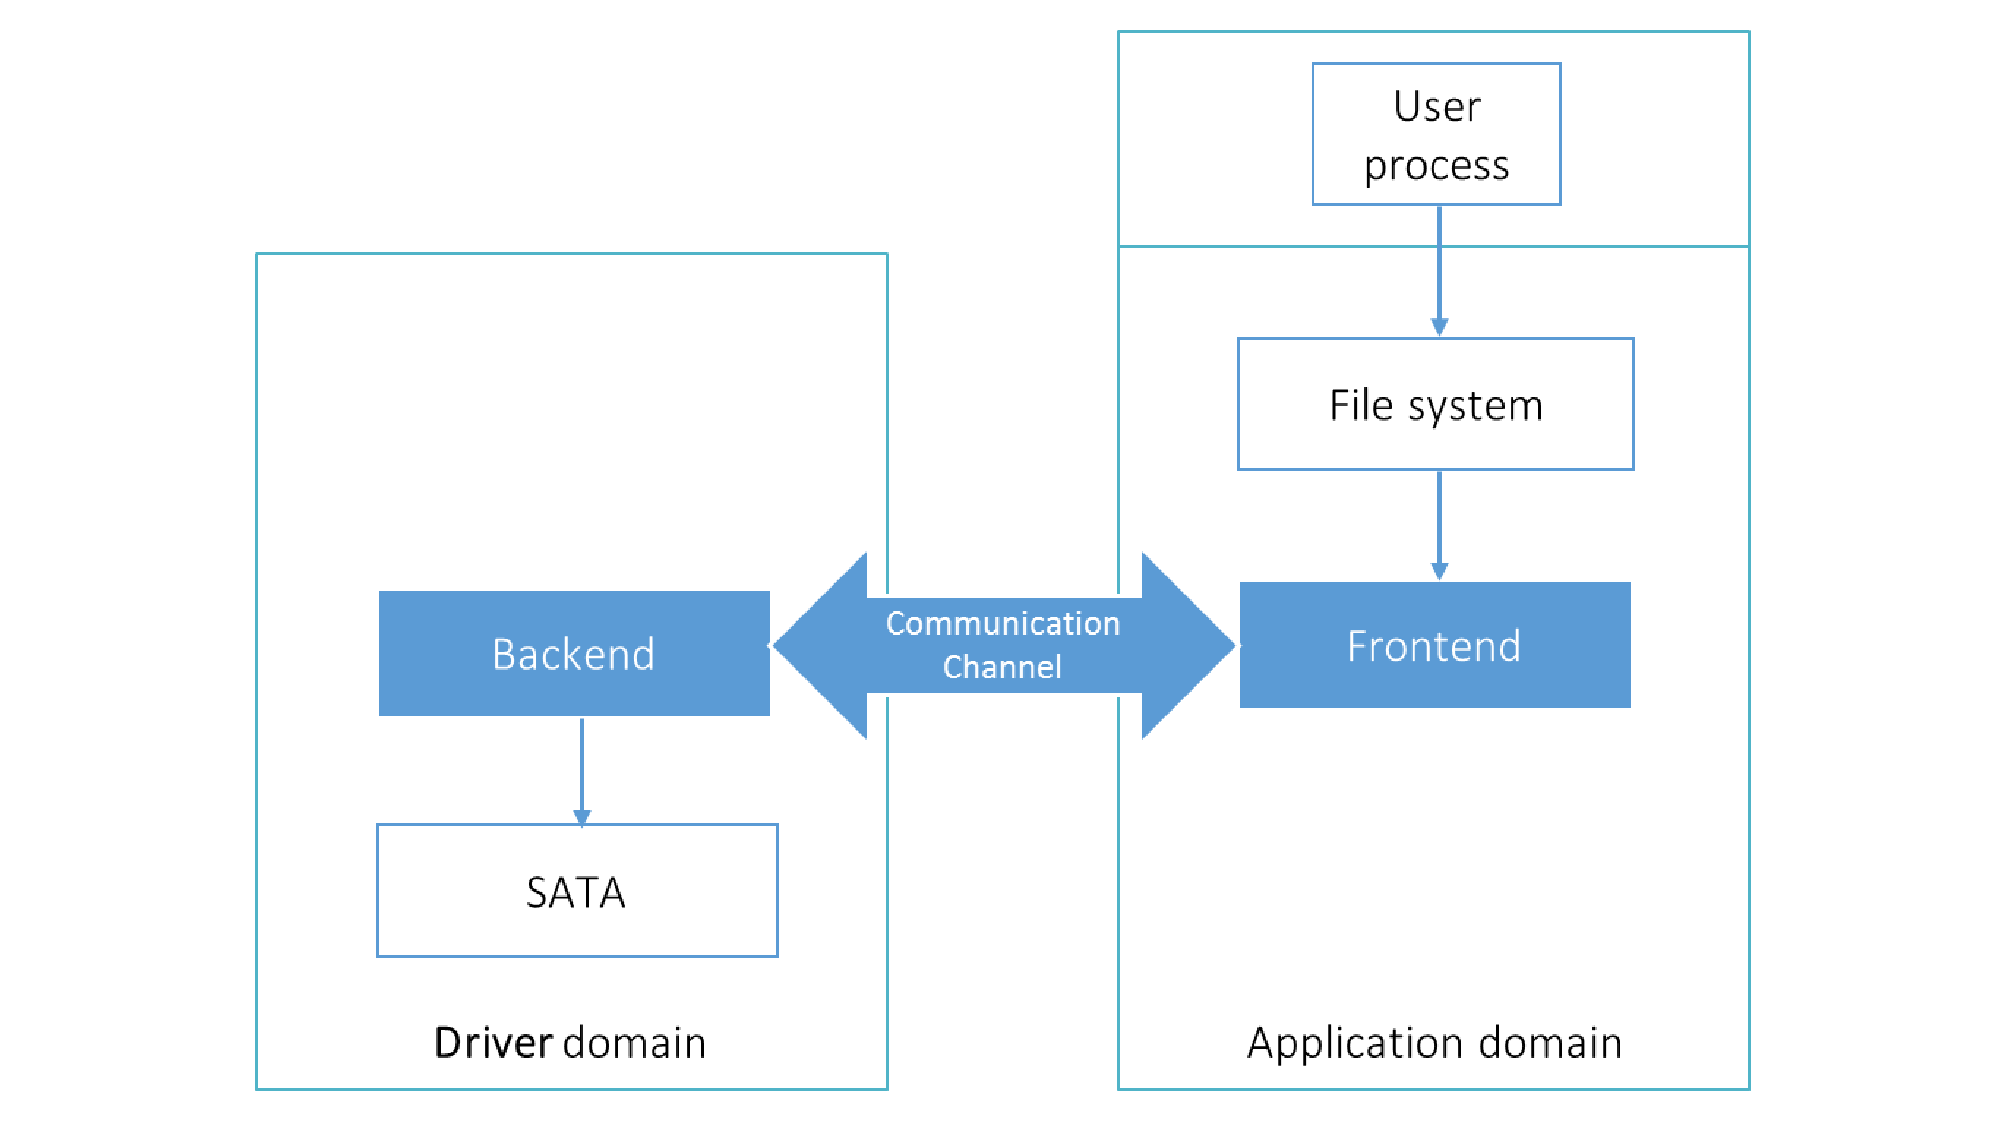
\includegraphics[scale=.5]{IDDRcomponents}
\caption{System Components}
\label{fig:Design Evo1}
\end{figure}

\subsection{Front end driver}
\label{subsec:frontend}
As mentioned earlier in section~\ref{sec:properties}, transperency is one the properties of the IDDR, which requires us to avoid any changes to the kernel as well as the device driver. In the IDDR, the device driver runs in the driver domain and the user applications run in the application domain. Hence, the user application will not know about the device driver execution in the driver domain. Thus, it is not possible for the application to send requests to the driver in the driver domain, without making any changes to the kernel. As a result, IDDR runs a piece of a code called \textit{front end} in an application domain. The front end driver acts as a substitute for the device driver. The main functionality of the front end driver is to accept requests from the user application, process the requests, enqueue the requests for the driver domain and notify the driver domain. It also takes care of the processing of the responses and ending the corresponding requests.

\subsection{Back end driver}
\label{subsec:backend}
The kernel and the device driver provide a functionality to accept requests from the user application running in the same domain. The kernel is not capable of accepting the requests from the application running in a separate domain without making any changes to the kernel code. At the same time, device driver is not capable of sending responses back to the application domain without making any changes to the device driver code. In order to avoid making any changes to the device driver and kernel, a piece of code called the \textit{back end driver} runs in the driver domain. The responsibility of a back end driver is to accept requests from the application domain and forward them to the device driver. The back end driver sends the responses and notifies the application domain after receiving the responses from the device driver.
\begin{figure}[!ht]
\centering
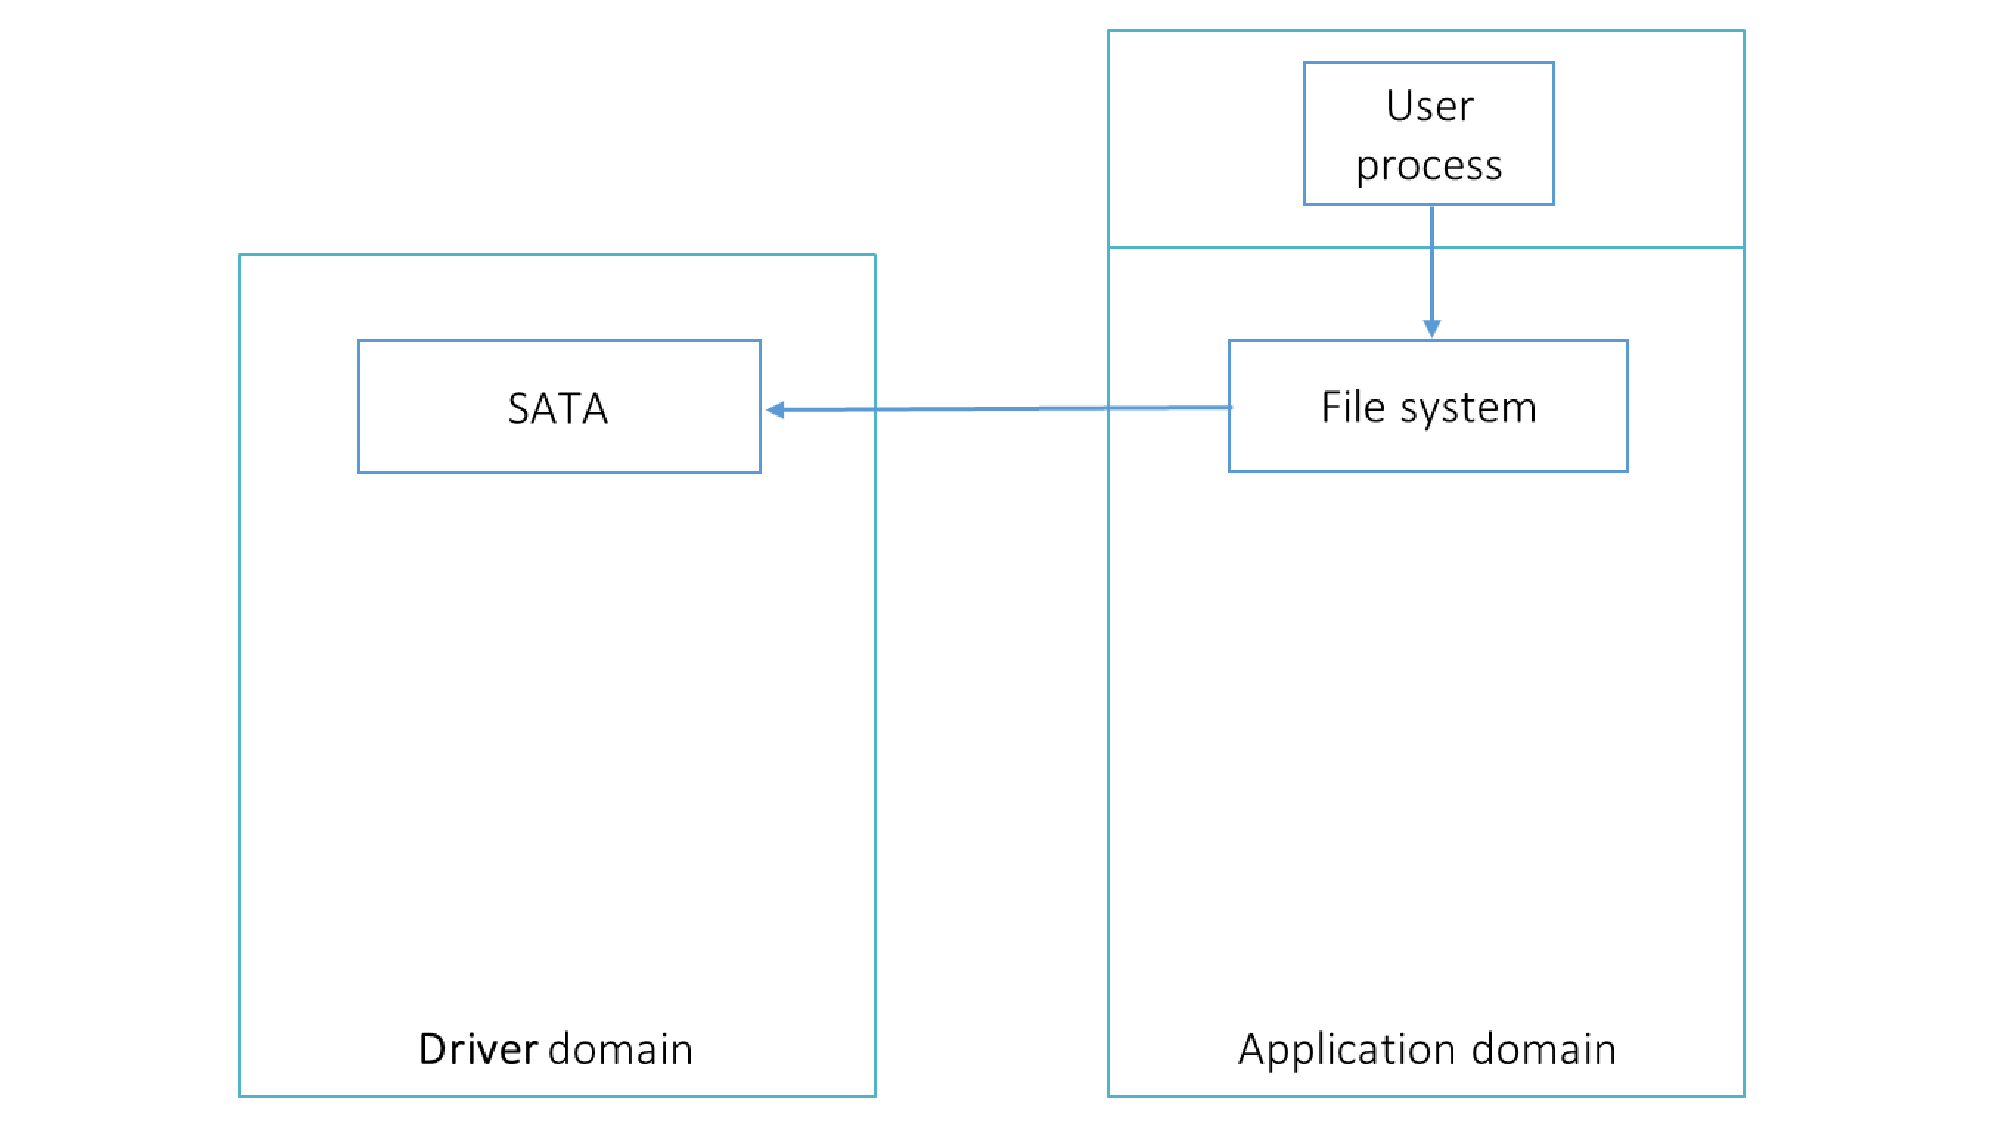
\includegraphics[scale=.5]{component1}
\caption{Conceptual design of driver domain}
\label{fig:conept}
\end{figure}
\begin{figure}[!ht]
\centering
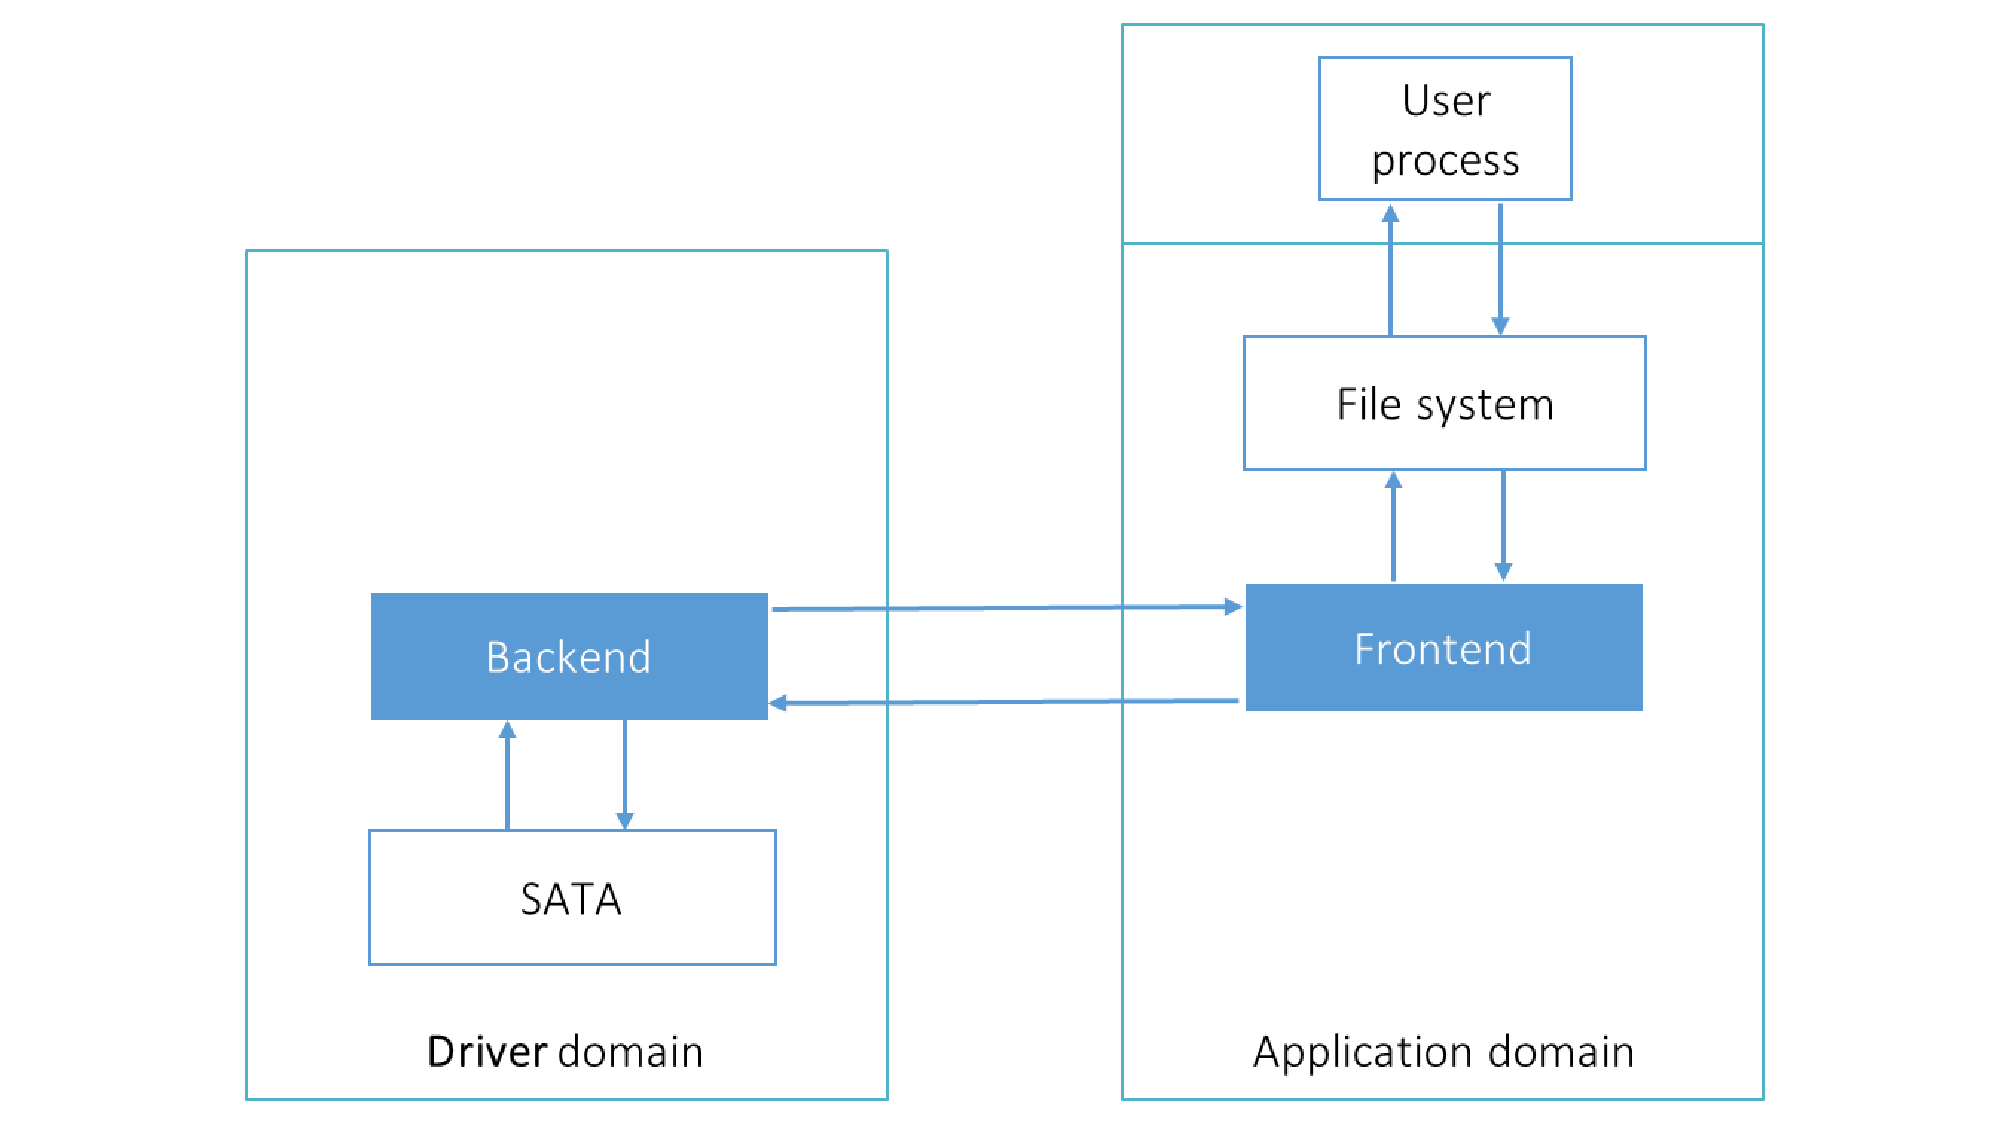
\includegraphics[scale=.5]{component2}
\caption{Back end and front end drivers}
\label{fig:backendfrontend}
\end{figure}

\subsection{Communication module}
The communication module is a communication channel between the front end driver and the back end driver. Unlike the back end and the front end driver, the communication module is not a separate physical entity or a kernel module. The communication channel exists in the front and the back end driver. It is logically divided into three parts. The responsibility of the first part is to forward the requests from the application domain to the driver domain as well as to forward the responses from the driver domain to the application domain. The responsibility of the second part is to share the read and write data and the responsibility of the third part is to notify the other domain upon the occurrence of a particular event. 

Figure~\ref{fig:communication} illustrates the role of the communication model. 
\begin{figure}[!ht]
\centering
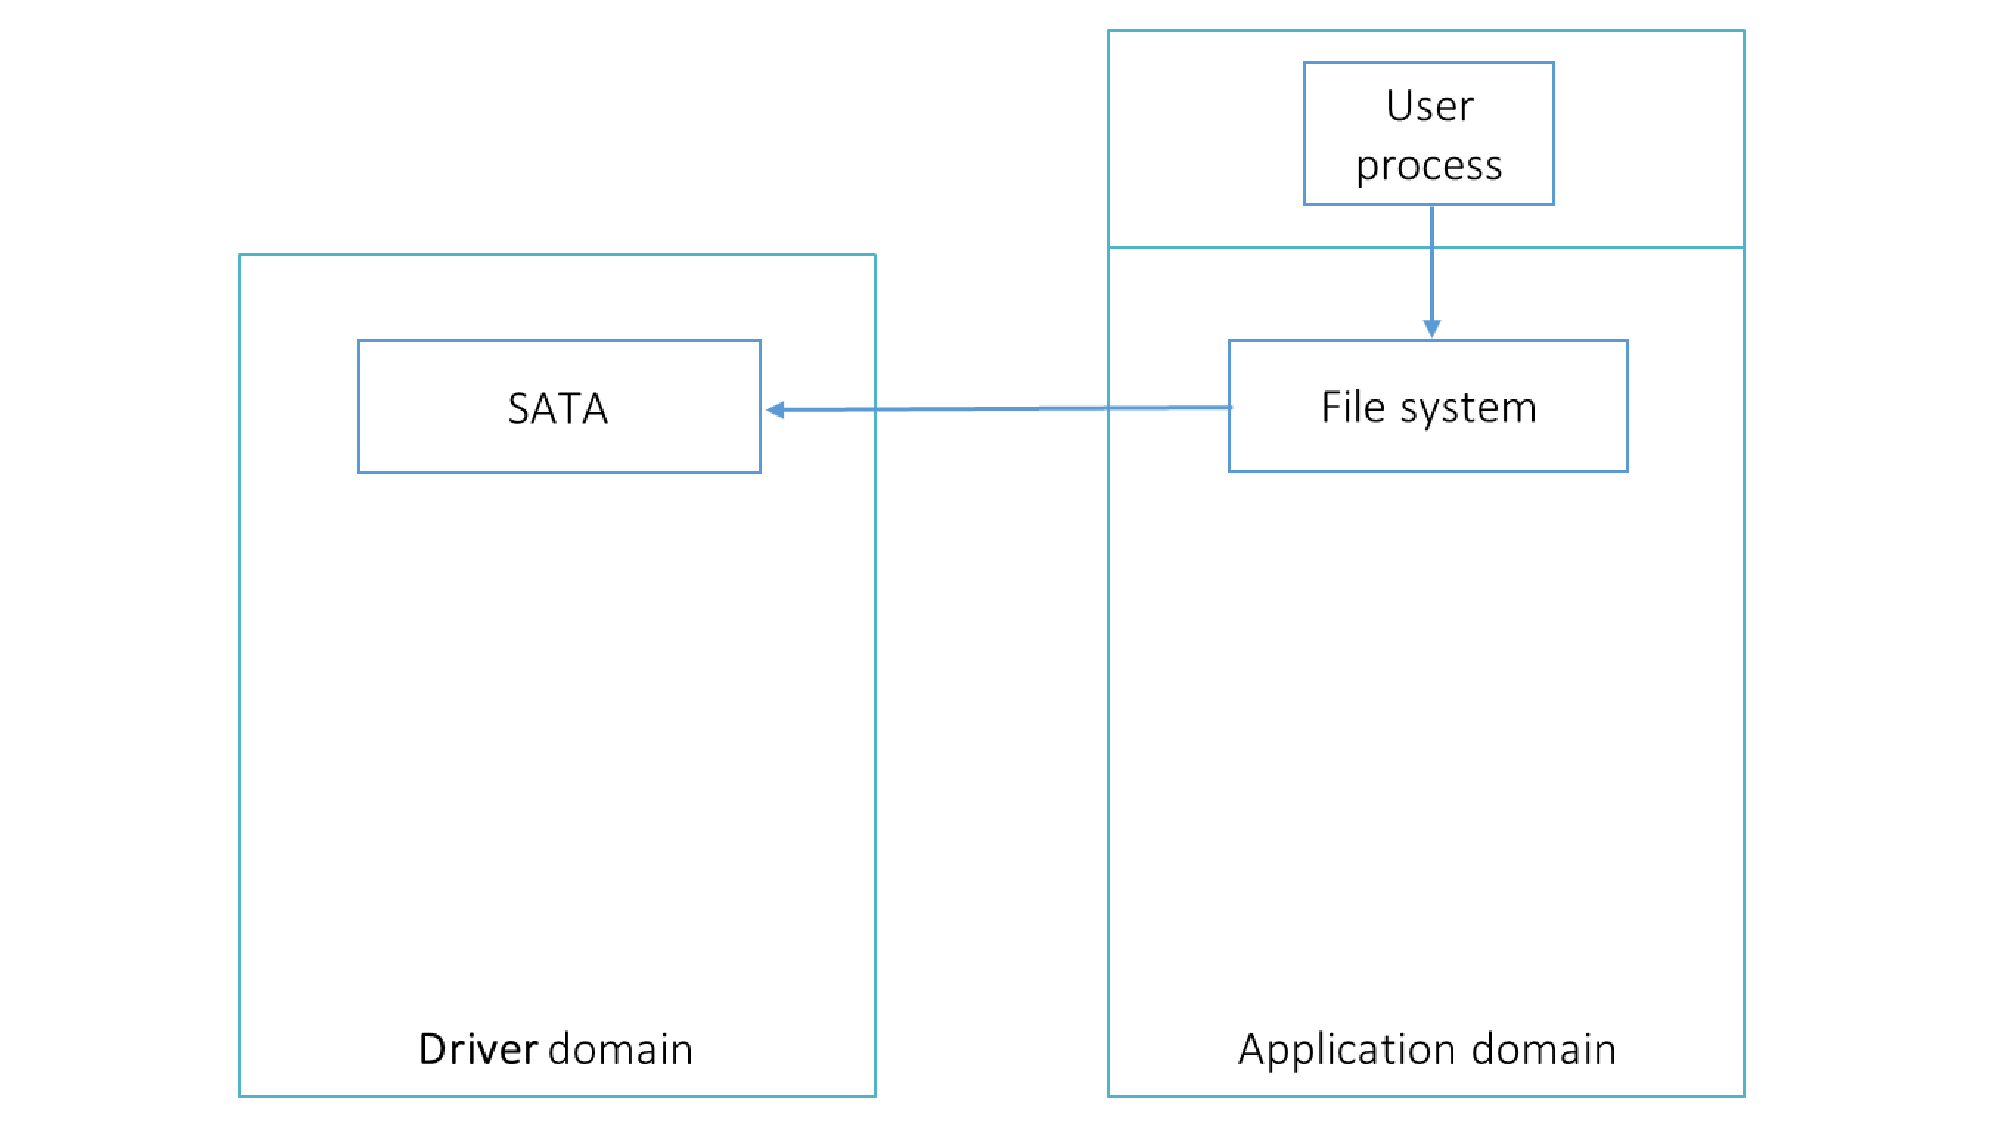
\includegraphics[scale=.5]{component1}
\caption{Communication module}
\label{fig:communication}
\end{figure}
\pagebreak

\section{System design}\label{design}
\begin{figure}[!ht]
\centering
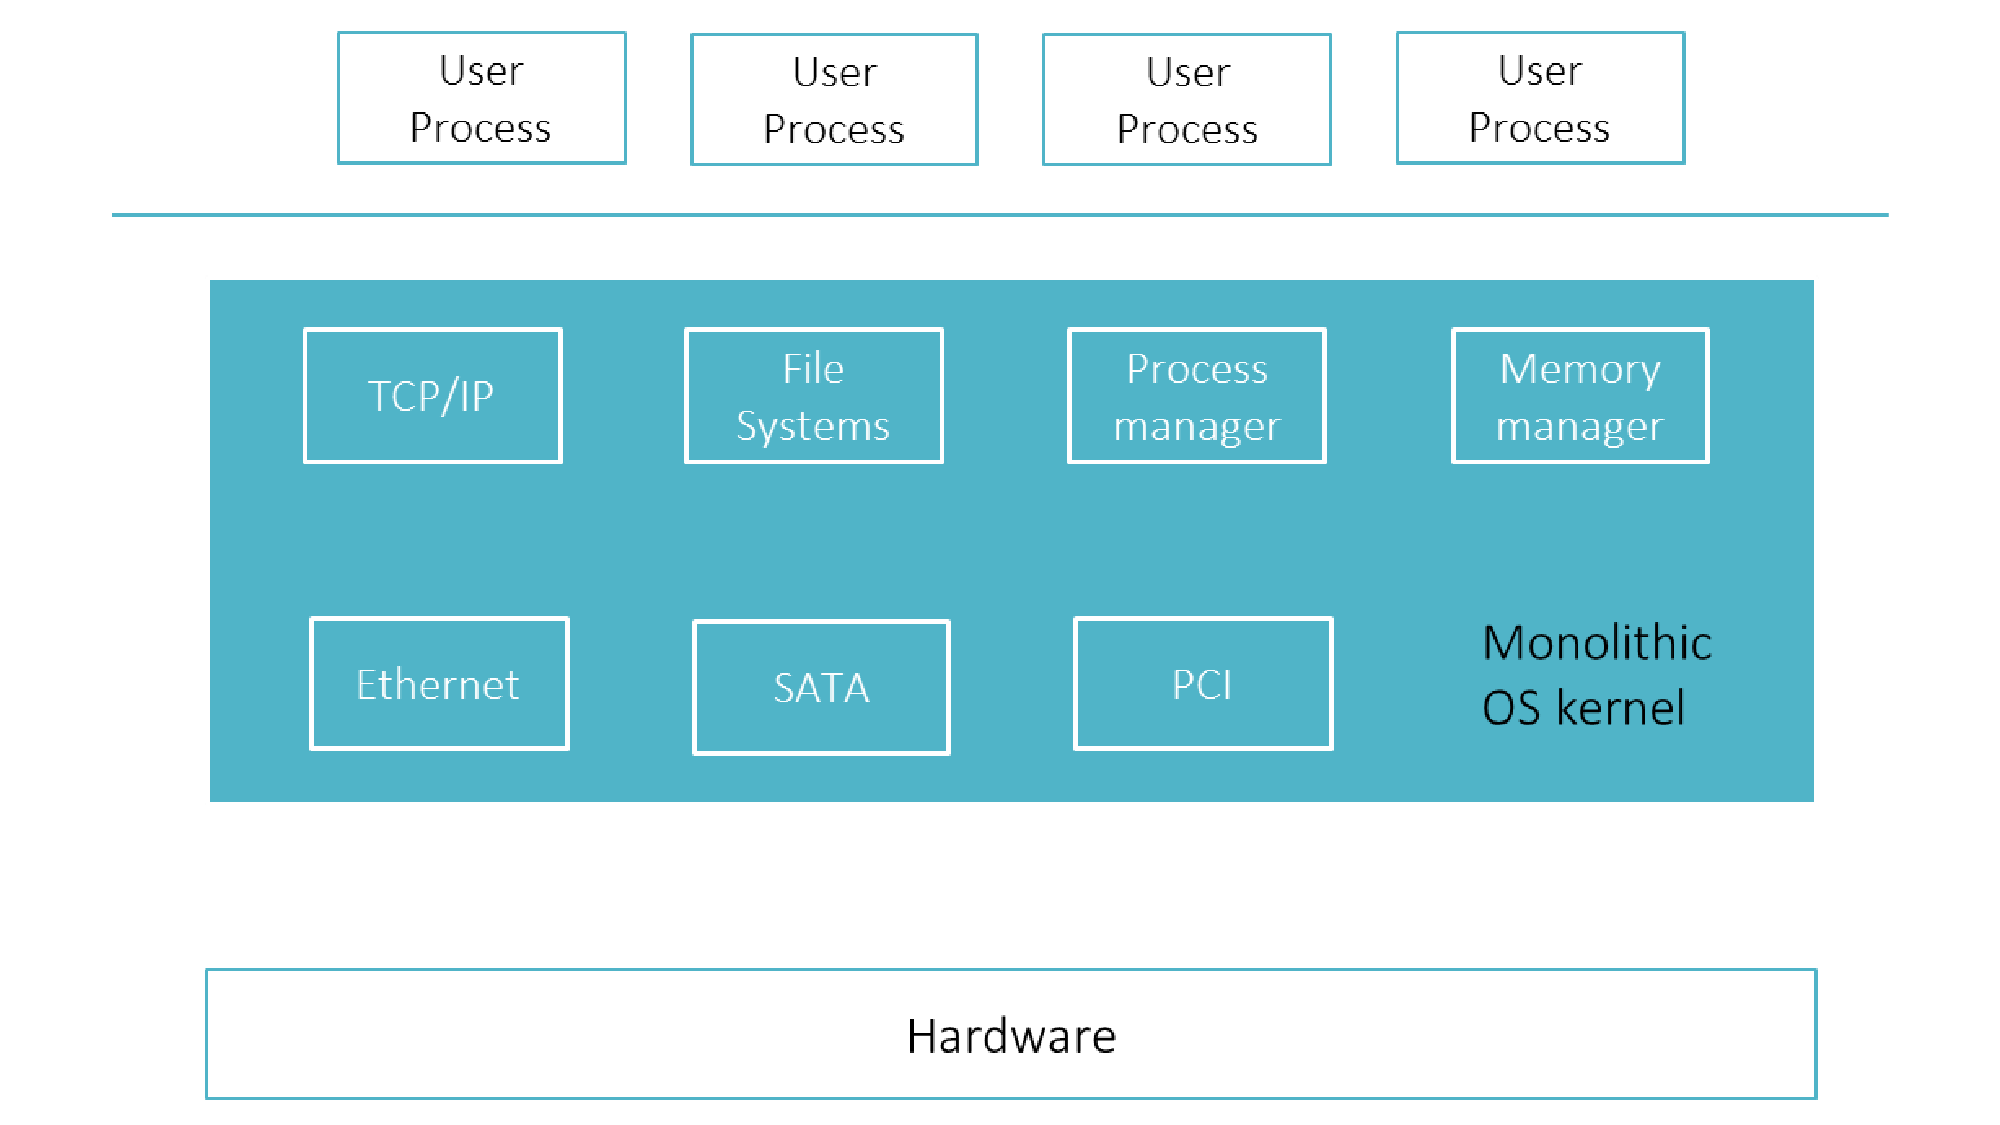
\includegraphics[scale=.5]{OSoverview}
\caption{Tightly coupled System}
\label{fig:monolithic}
\end{figure}
Figure~\ref{fig:monolithic} shows the architectural overview of the modern operating system with a monolithic kernel and Figure~\ref{fig:isolated} illustrates the concept of the IDDR.
\begin{figure}[!ht]
\centering
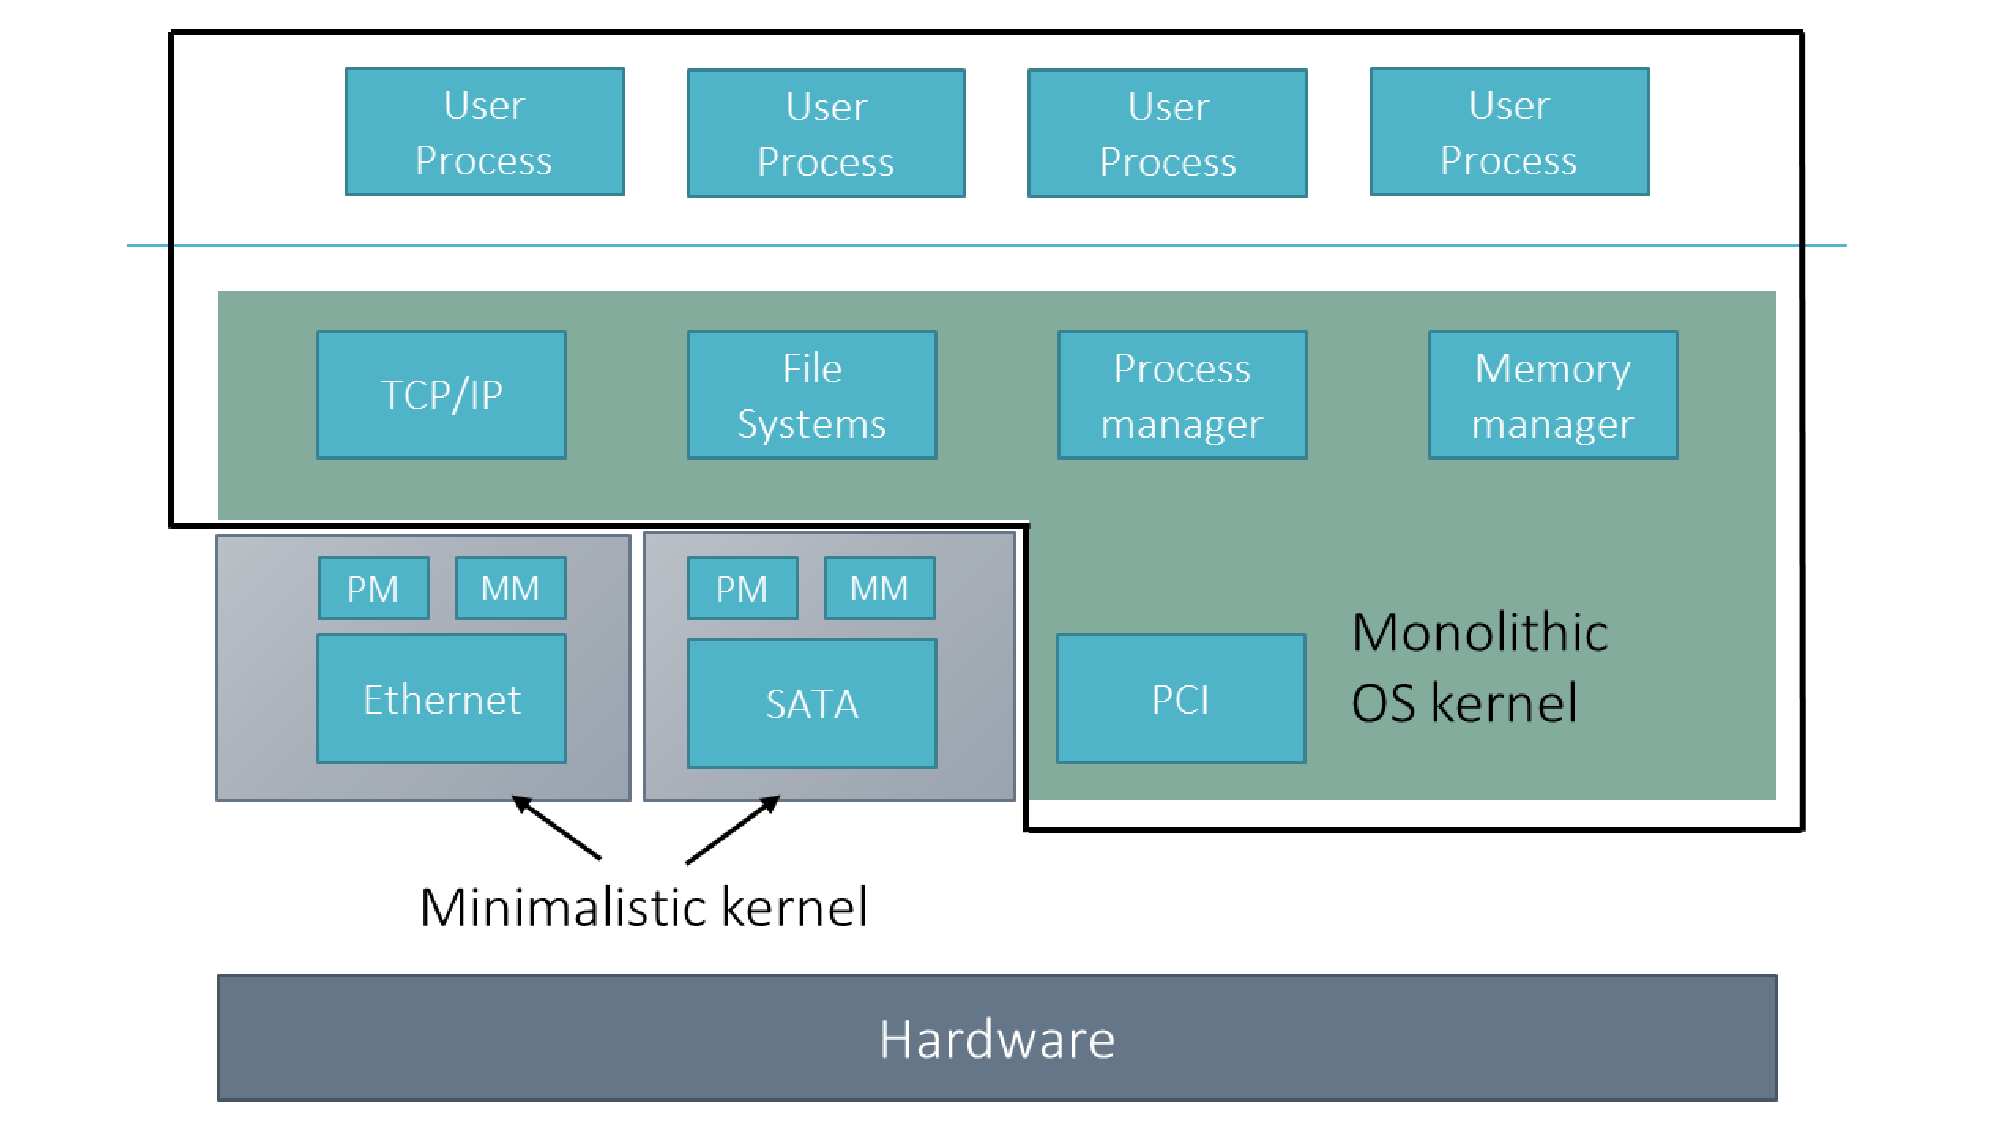
\includegraphics[scale=.5]{IDDRoverview}
\caption{System with kernel and isolated device driver}
\label{fig:isolated}
\end{figure}

The following section explains the design evolution of the IDDR in brief. 
\\
Although the solution to provide more protection at the kernel level is to isolate the device driver from the Linux kernel, it is not possible to run a standalone device driver. A device driver is dependent on the kernel components such as scheduler, memory management unit etc. Hence an instance of a minimalistic kernel runs with the device driver removing the dependency. 
\\
Even though a device driver can be isolated from Linux kernel by running it with a new instance of minimalistic kernel, it is not possible to run multiple kernels over the same hardware without any virtual machine monitor. Thus, virtualization is used for running multiple monolithic kernels on a virtual machine monitor.
\\
Figure~\ref{fig:driver crash} and Figure~\ref{fig:high avail} explains the effects of a malicious activity occurring in the device driver isolated from the Linux kernel. When a device driver running in a driver domain hits a bug, it crashes the kernel of the driver domain and hence the driver domain itself. In addition, applications expecting a response from the driver domain might hang or crash waiting for the response. But due to the address space separation of the application domain and the driver domain, the application domain will remain intact.   
\begin{figure}[!ht]
\centering
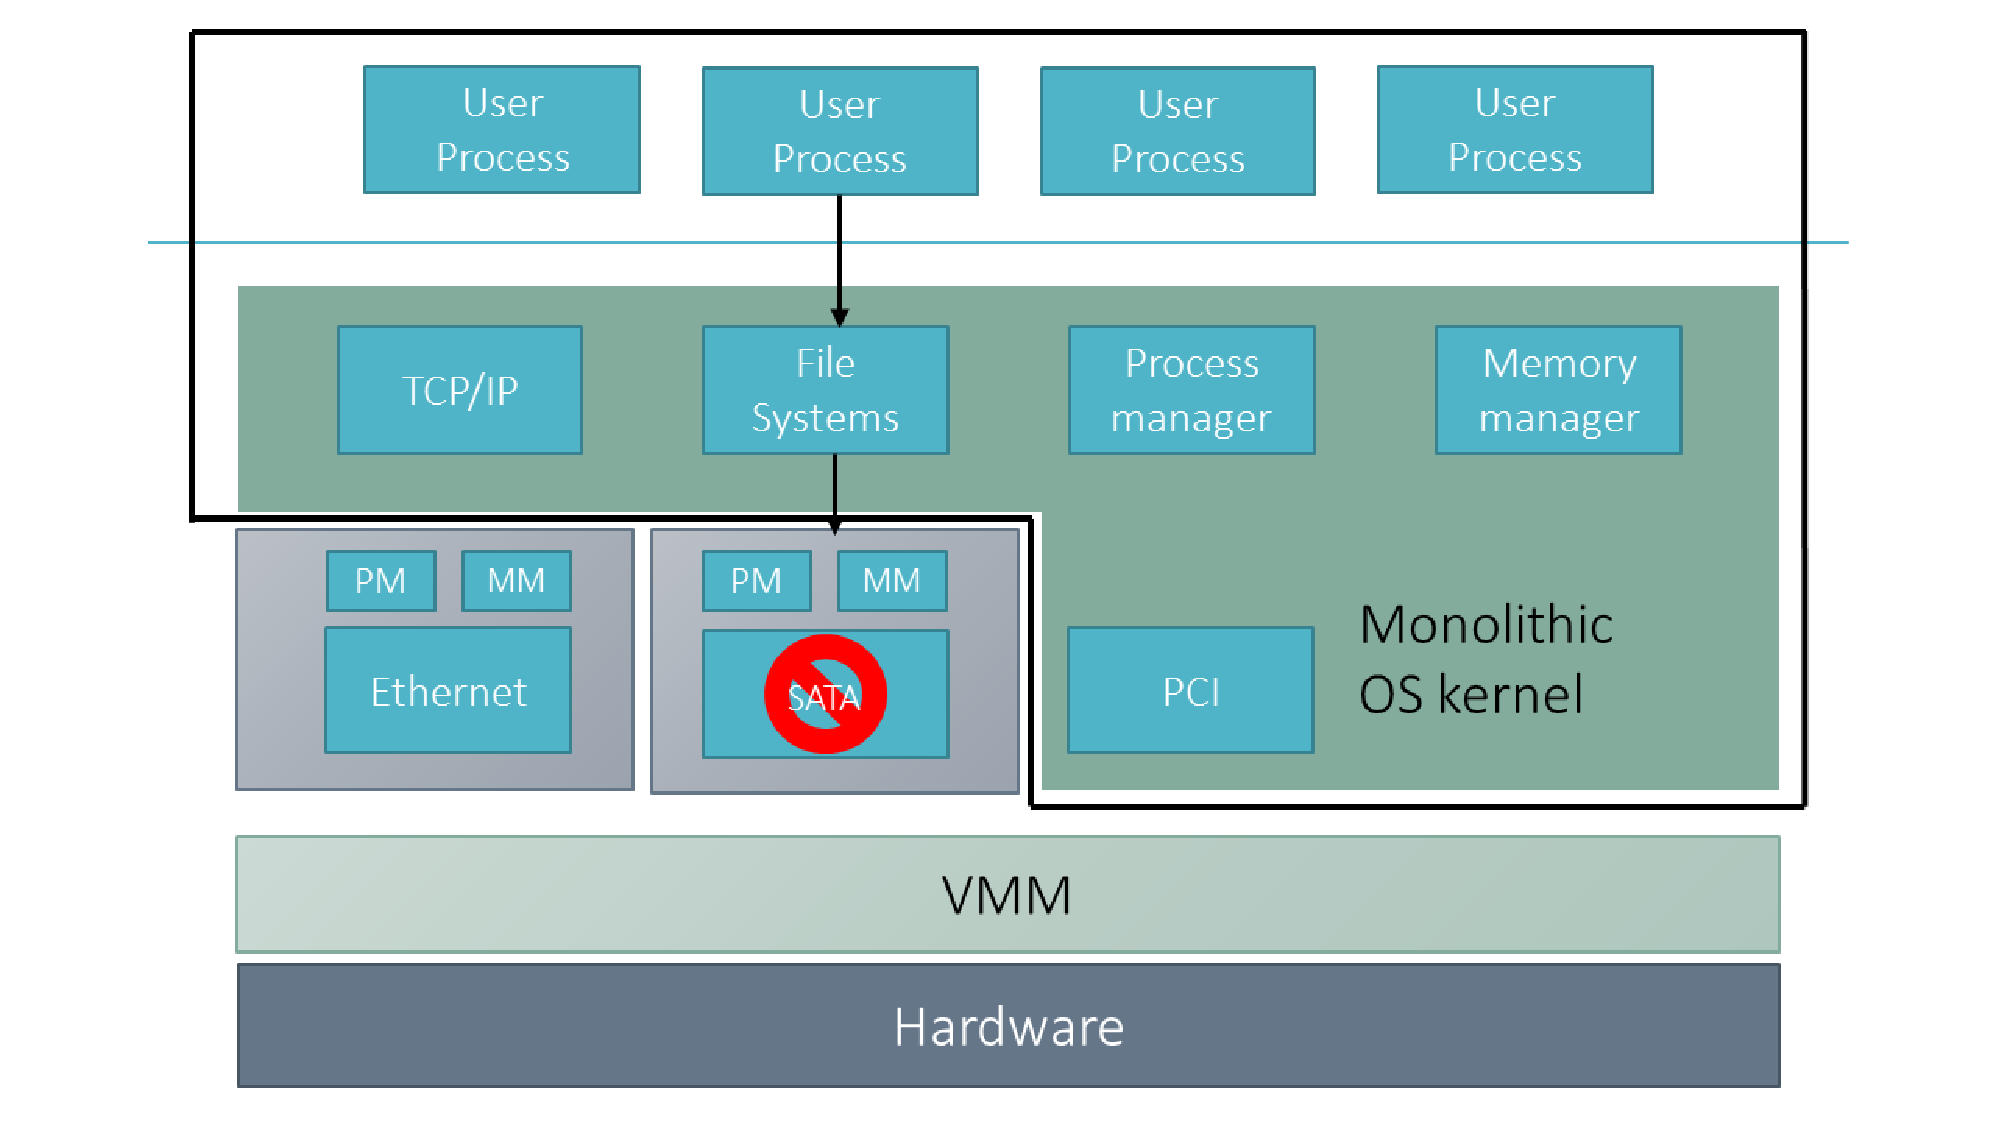
\includegraphics[scale=.5]{IDDRcrash1}
\caption{Device driver crash}
\label{fig:driver crash}
\end{figure}
\begin{figure}[!ht]
\centering
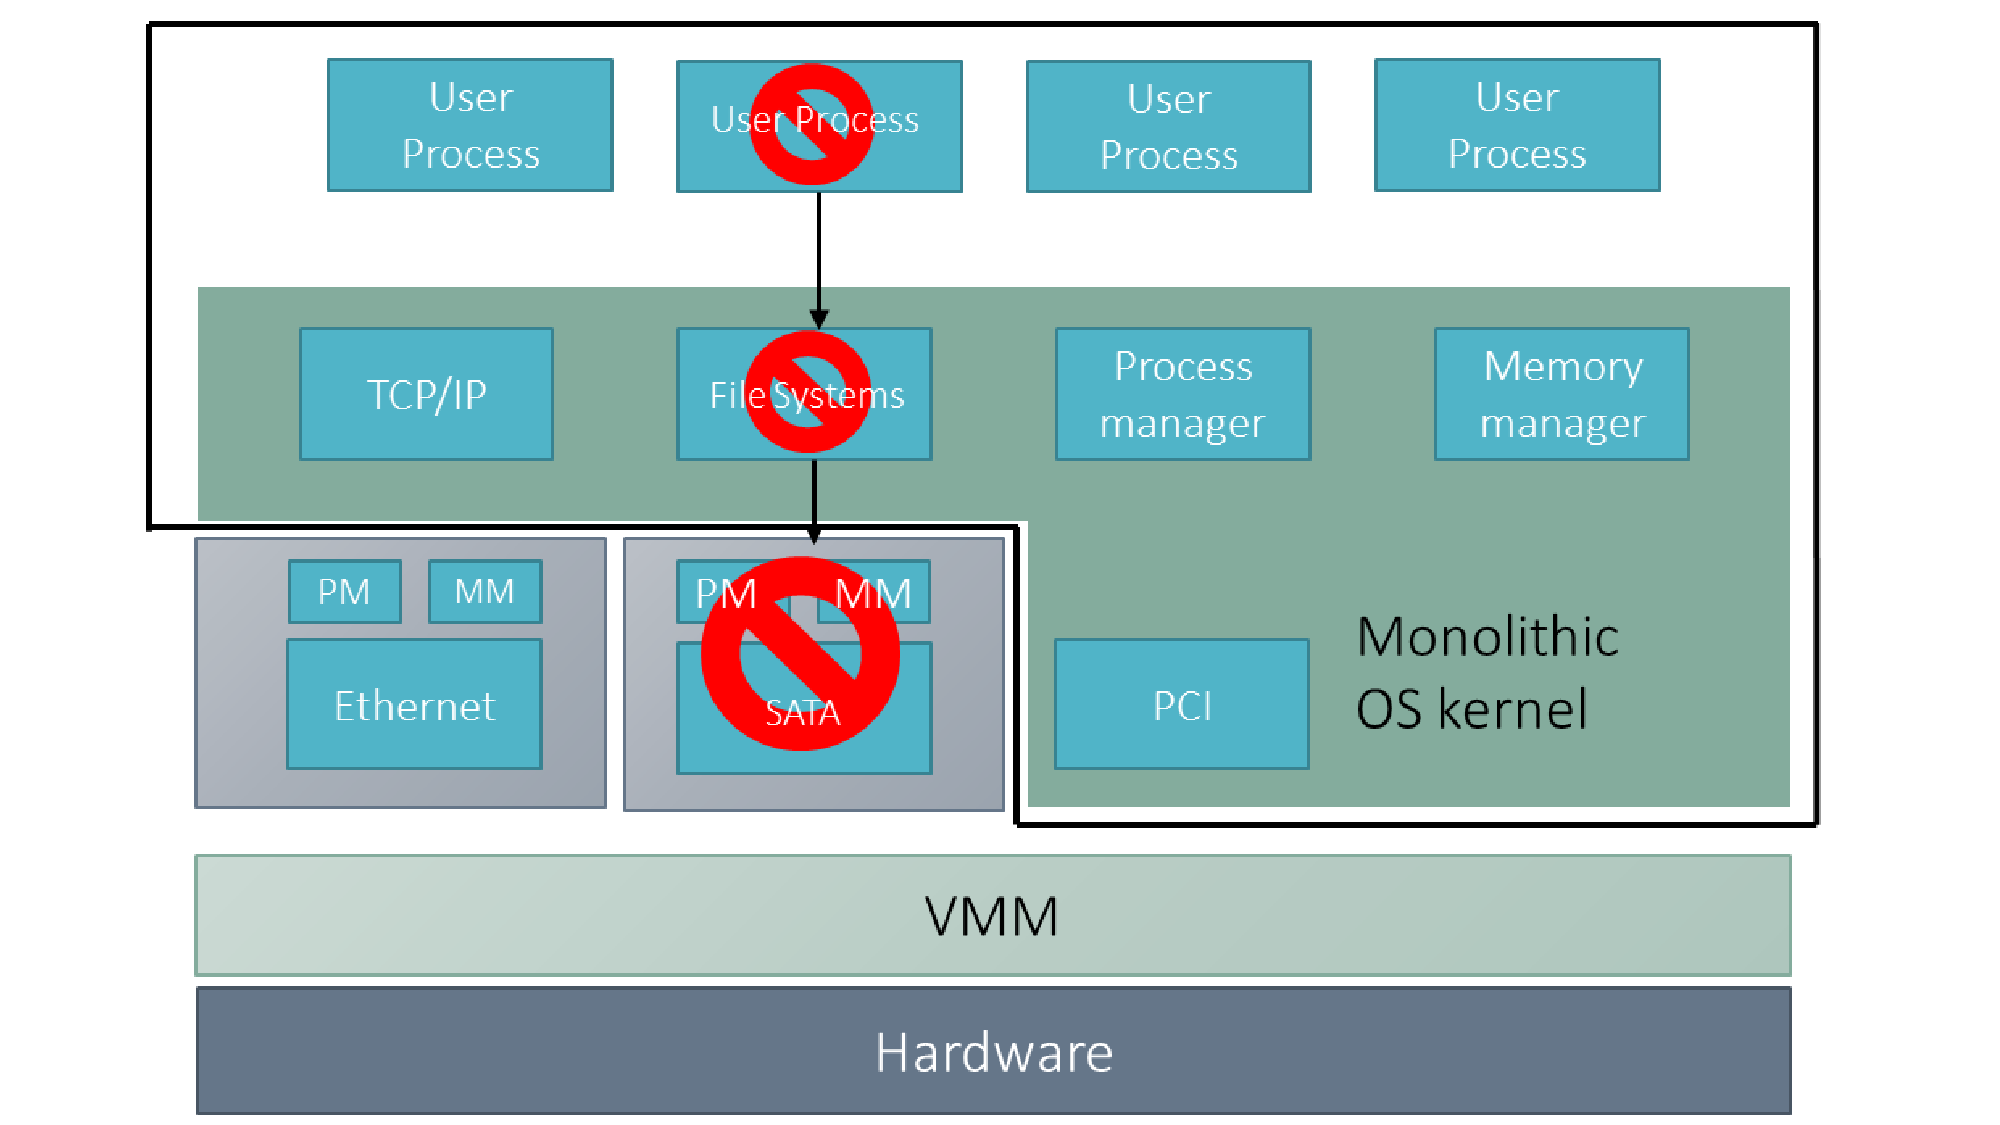
\includegraphics[scale=.5]{IDDRcrash2}
\caption{High Availability}
\label{fig:high avail}
\end{figure}
\pagebreak
    
\ifbool{toShowBibliography}{\bibliography{references}}{}
